\section{Methods}
Our method models two types of signal from the data -- change in number of fragments sequenced from a particular genomic region, and change of the allele distributions at SNP loci. In what follows, we first describe each signal processing separately and later show how we combine them into a joint prediction of fetal CNVs.

\todo[inline]{describe inheritance patterns and phased patterns here}

\subsection{SNP allele distribution}
For every SNP locus we observe a distribution of nucleotides in maternal plasma reads mapping to this particular position. Here we focus on calculating the probability of the observation w.r.t. a phased inheritance pattern. Formally, for observed 4-tuple $\(k_\A, k_\C, k_\G, k_\T\)$ of number of occurrences of each nucleotide, and phased inheritance pattern $\PP$ we model the conditional probability as Poisson distribution approximated by a Gaussian, i.e.
\begin{align*}
Pr[\(k_\A, k_\C, k_\G, k_\T\) ~|~ \text{mat. haplotypes } M_A, M_B; \text{pat. haplotypes } P_A, P_B; \text{admixture } r; \PP] \sim \N\(\vmu, \vSigma \)
\end{align*}
where
\begin{align*}
\vmu =&~ \(\mu_\A, \mu_\C, \mu_\G, \mu_\T\) \\
\vSigma =&~ \vmu \mathbf{I}_4
\end{align*}
To compute $\mu_x, x \in \{\A,\C,\G,\T\}$, we first adjust the mixture ratio $r$  based on phased pattern $\PP$ to reflect the expected number of fetal haplotypes $|H_\PP|$. 
\begin{align*}
r' =&  \frac{ r/2 \cdot |H_\PP| }{r/2 \cdot |H_\PP| ~\cdot~ (1-r) }
\end{align*}
Then for each nucleotide $x$ we sum probabilities of all the possible sources it might have been sequenced from, which includes maternal haplotypes and fetal haplotypes:
\begin{align*}
p_x &= \sum_{i = A}^B (x \text{ equals } M_i) \cdot m_i (1-r')/2  \\
	&~~~ + \sum_{i = 1}^{|H_\PP|} (x \in H_\PP) \cdot r'/|H_\PP|  \\
\end{align*}
For reads putatively coming from indigenous maternal DNA, we correct for maternal CNVs by using the allele ratios $m_i$ as observed in maternal-only sequencing data. Additionally, in order to mitigate noise we add pseudocount $\alpha$ to these counts.
\begin{align*}
m_i &= \frac{\alpha + \# \text{reads supporting }M_i\text{ in maternal seqencing}}{2\alpha + \sum_{j=A}^{B}\# \text{reads supporting }M_j\text{ in maternal seqencing}}
\end{align*}
This way, we obtain the expected multinomial probability distribution over nucleotides aligned to this SNP locus in reads mapped to span this position. Thus to get the expected number of reads supporting particular variant at this SNP locus, we have to multiply $p_x$ by the number of reads mapped,
\begin{align*}
\mu_x &= p_x \cdot \#\text{mapped reads}
\end{align*}


\subsection{CNV calling based on sequencing coverage}
Sequencing of cell-free DNA carries sequencing biases other then just GC content when compared to standard WGS. ... \cite{srinivasan2013}

\subsection{Hidden Markov Model for CNVs Inference}\label{ss:hmm}
%To combine the signals form individual SNP positions, we use a hidden Markov model. For each inheritance pattern we use a model like in Figure \ref{fig:model}, to compute likelihood of the observed samples under assumption of such inheritance pattern. To the possible inheritance patterns correspond the states of the HMM (for each SNP position) with emission probabilities proportional to the likelihood. See Figure \ref{fig:hmm}. As the likelihood which we get from the graphical model is already probability, we can interpret it right away as the emission probability. In practice we add some small positive constant $\varepsilon$ to these probabilities (and then normalize) to account for noise in the data.

%\begin{figure}[h!]
%\missingfigure{HMM}
%\center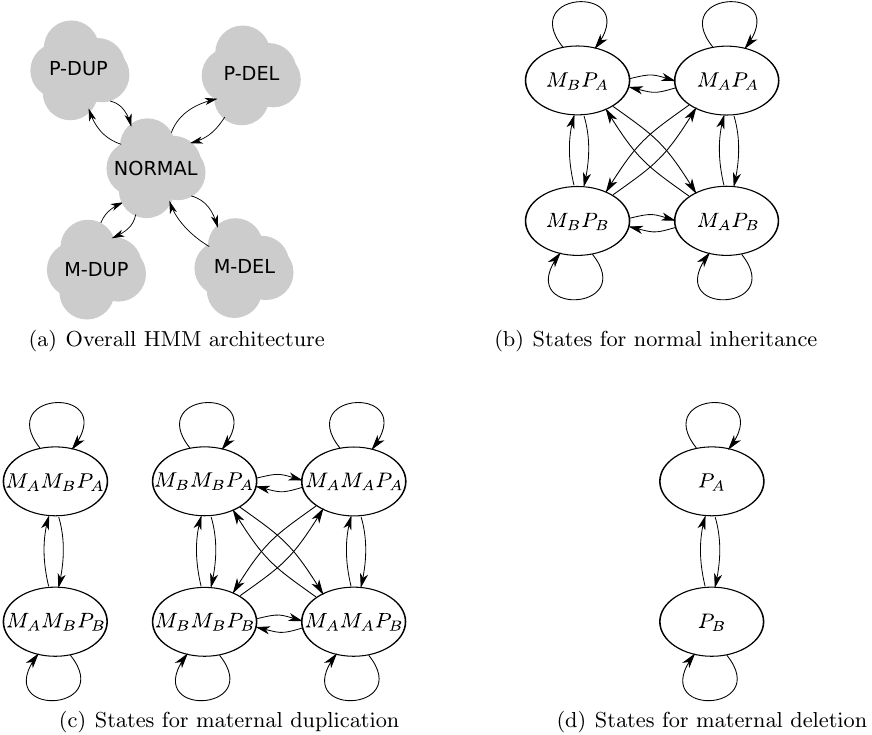
\includegraphics[width = 0.95\textwidth]{hmm}
%\caption{Hidden Markov model used for CNV inference. We do not allow two CNVs to be adjacent, thus the switching always has to go through ``1M 1P'' (normal) state. The thicker arrows signalize higher transition probability to stay in the particular inheritance pattern.}\label{fig:hmm}
%\end{figure}

%The HMM as depicted in Figure \ref{fig:hmm} is in a more general form, when we allow for different transition probabilities, depending on the given SNP site. This is useful if we want to model for non-uniform distance between individual SNPs. However in this project we assume uniform distribution and thus the transition probabilities are independent of actual position.
